\documentclass[tikz,border=3mm]{standalone}
\usetikzlibrary{positioning, shapes, arrows, arrows.meta}

\begin{document}
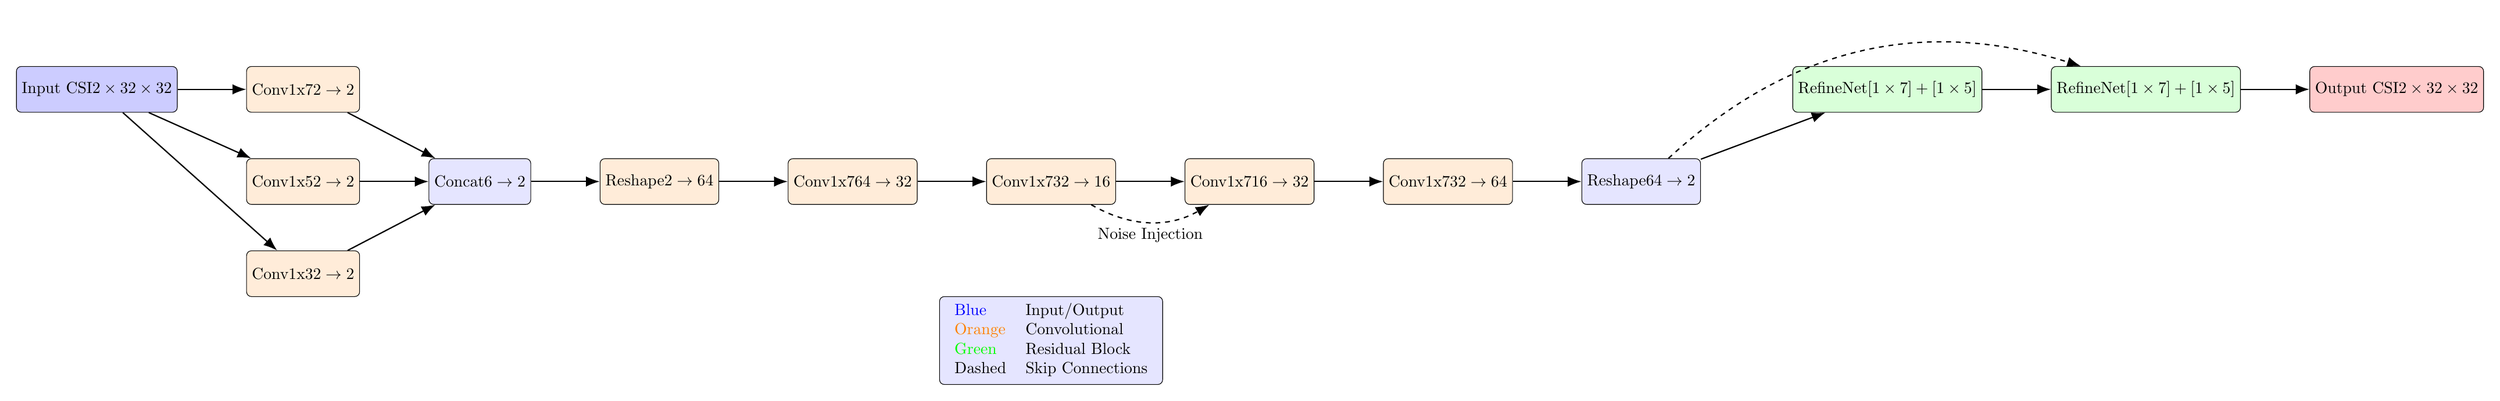
\begin{tikzpicture}[
    node distance=1cm and 1.5cm,
    block/.style={draw, fill=blue!10, rectangle, minimum width=2cm, minimum height=1cm, rounded corners=3pt},
    conv/.style={block, fill=orange!15},
    residual/.style={block, fill=green!15},
    arrow/.style={-{Latex[length=3mm]}, thick}
]

% Input
\node[block, fill=blue!20] (input) {Input CSI \\ $2\times32\times32$};

% Encoder Paths
\node[conv, right=of input] (conv1x7) {Conv1x7 \\ $2\rightarrow2$};
\node[conv, below=of conv1x7] (conv1x5) {Conv1x5 \\ $2\rightarrow2$};
\node[conv, below=of conv1x5] (conv1x3) {Conv1x3 \\ $2\rightarrow2$};

% Concatenation
\node[block, right=of conv1x5] (concat) {Concat \\ $6\rightarrow2$};

% Latent Space
\node[conv, right=of concat] (reshape) {Reshape \\ $2\rightarrow64$};
\node[conv, right=of reshape] (encoder1) {Conv1x7 \\ $64\rightarrow32$};
\node[conv, right=of encoder1] (encoder2) {Conv1x7 \\ $32\rightarrow16$};

% Decoder
\node[conv, right=of encoder2] (decoder1) {Conv1x7 \\ $16\rightarrow32$};
\node[conv, right=of decoder1] (decoder2) {Conv1x7 \\ $32\rightarrow64$};
\node[block, right=of decoder2] (reshape2) {Reshape \\ $64\rightarrow2$};

% RefineNet
\node[residual, above right=1cm and 2cm of reshape2] (refine1) {RefineNet \\ $[1\times7]+[1\times5]$};
\node[residual, right=of refine1] (refine2) {RefineNet \\ $[1\times7]+[1\times5]$};

% Output
\node[block, fill=red!20, right=of refine2] (output) {Output CSI \\ $2\times32\times32$};

% Arrows
\draw[arrow] (input) -- (conv1x7);
\draw[arrow] (input) -- (conv1x5);
\draw[arrow] (input) -- (conv1x3);
\draw[arrow] (conv1x7) -- (concat);
\draw[arrow] (conv1x5) -- (concat);
\draw[arrow] (conv1x3) -- (concat);
\draw[arrow] (concat) -- (reshape);
\draw[arrow] (reshape) -- (encoder1);
\draw[arrow] (encoder1) -- (encoder2);
\draw[arrow] (encoder2) -- (decoder1);
\draw[arrow] (decoder1) -- (decoder2);
\draw[arrow] (decoder2) -- (reshape2);
\draw[arrow] (reshape2) -- (refine1);
\draw[arrow] (refine1) -- (refine2);
\draw[arrow] (refine2) -- (output);

% Skip connections
\draw[arrow, dashed] (encoder2) to[bend right] node[midway, below] {Noise Injection} (decoder1);
\draw[arrow, dashed] (reshape2) to[bend left] (refine2);

% Legend
\node[block, below=2cm of encoder2] (legend) {
    \begin{tabular}{ll}
        \textcolor{blue}{Blue} & Input/Output \\
        \textcolor{orange}{Orange} & Convolutional \\
        \textcolor{green}{Green} & Residual Block \\
        Dashed & Skip Connections
    \end{tabular}
};

\end{tikzpicture}
\end{document}